\chapter{基础操作}
\label{cha:基础操作}

\section{机器人上电}

操作前,请再次确认已阅读并确保已遵循\prettyref{sec:安全指南} 内容,排除潜在风险,确保操作安全。

\begin{figure}[hb]
    \centering
    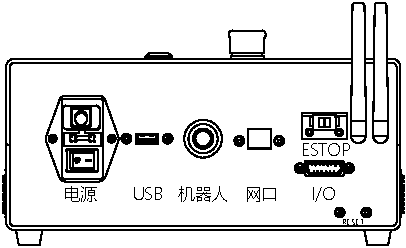
\includegraphics[height=5cm]{line_graphs/robot_control_box_back.pdf}
    \caption{控制箱背板示意图}
    \label{fig:控制箱背板示意图}
\end{figure}

\begin{enumerate}
\item 将机器人电缆插头插入控制箱的机器人接口。
\item 控制箱插上电源线,并将电源插头接入$\!220 \unit{V}\!$交流电插座。
\item 确保控制箱顶部的急停按钮处于释放\footnote{当急停按钮处于弹起状态时为释放状态,反之处于按下状态为锁定状态。}状态。
\item 打开控制箱背板的红色总电源开关,开关指示灯亮。
\item 长按(约3 秒)控制箱顶部的开关机按钮或外接开关机按钮(选配),直至控制箱顶部的开关机按钮的指示灯变成蓝色常亮,等待机器人肩部灯光亮起,完成控制箱和机器人的上电操作。
\end{enumerate}

    %  \footnotetext[a]{当使用$100\sim 200\unit{V}$ 供电时}
    %  \footnotetext[b]{当使用$200\sim 240\unit{V}$ 供电时}
\danger{\begin{itemize}
\item 请确保控制箱电源的插线板务必良好接地。
\item 请确保控制箱电源的输入电流受到漏电保护装置和适当的过流断路保护装置的保护。
\item 请确保所有的电缆在控制箱通电前都正确连接,始终正确使用原装的电源线。
\end{itemize}}

\danger[警告]{\begin{itemize}
\item 禁止在机器人启动时断开或用力拉拽机器人电缆。
\item 禁止延长或改动机器人电缆。
\item 切勿损坏电源线,或将重物压在电源线上。
\item 切勿使用破损或不符合的插座。
\item 切勿让电源插头和插座粘附灰尘或金属附着物。
\end{itemize}}

% \clearpage

\section{连接机器人}
LM3支持有线网络连接和无线网络连接,无线网络连接目前仅支持接入控制箱内置的Wi-Fi热点网络。
\subsection{有线网络连接}

如\prettyref{fig:有线网络连接拓扑图},使用网线连接控制箱背板的网口与路由器或交换机的LAN口,同时确保用于操作机器人的电脑、平板、手机或其他图形化终端设备与机器人接入的是同一网络。

\begin{figure}[ht]
    \centering
    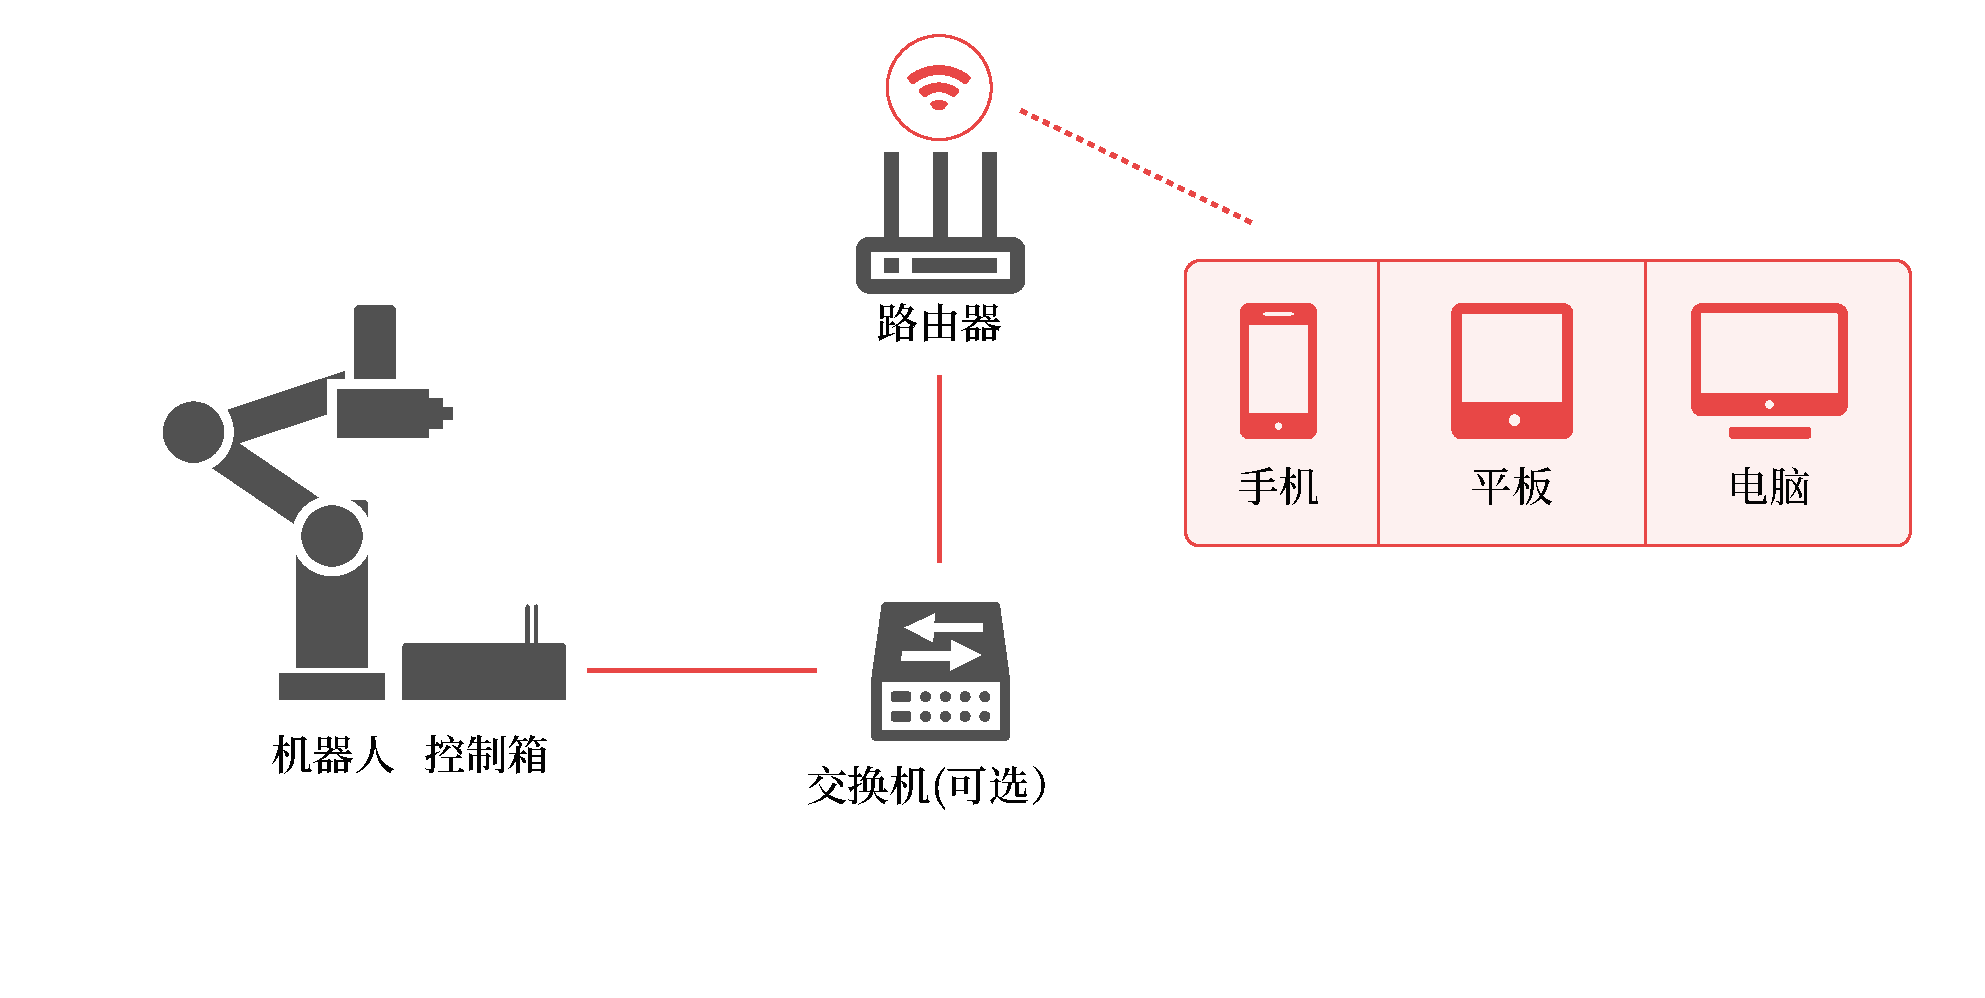
\includegraphics[width=\textwidth]{image/network-1.pdf}
    \caption{有线网络连接拓扑图}
    \label{fig:有线网络连接拓扑图}
\end{figure}

% \clearpage

\subsection{无线网络连接}
机器人出厂后,默认会启用一个热点名称为设备名称\footnote{可在控制箱的铭牌上找到设备名称。}的Wi-Fi热点,设备名称格式如:\verb|Lebai-123456|(后6位为随机字符),默认密码为:\verb|88888888|(8个8)。可通过电脑、平板、手机或其他图形化终端设备的Wi-Fi功能连接该设备名称对应的Wi-Fi热点网络,连接和控制机器人。

在设置页面修改设备昵称,会修改设备的 SSID。

\begin{figure}[ht]
    \centering
    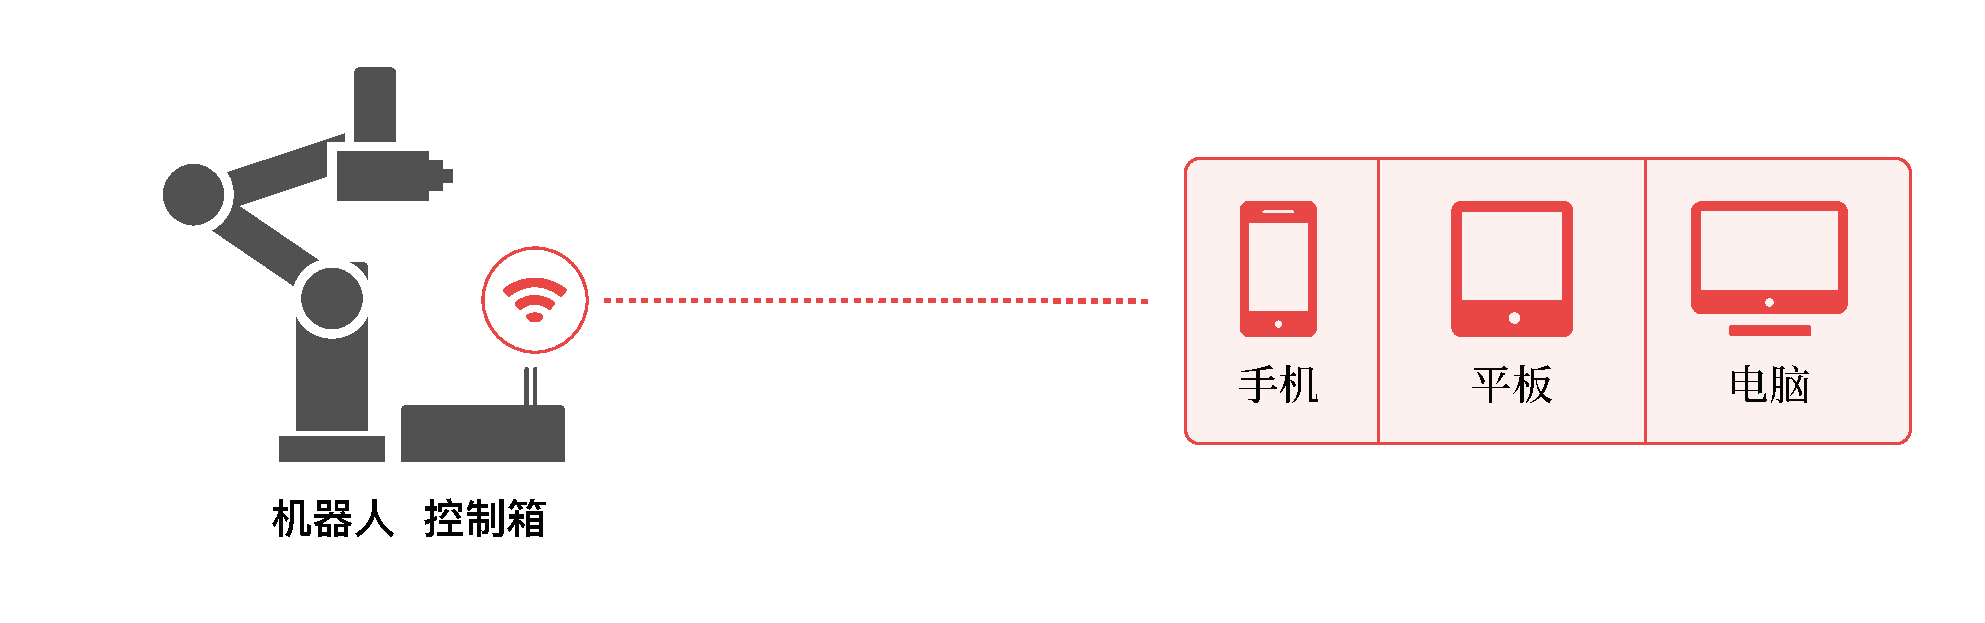
\includegraphics[width=\textwidth]{image/network-2.pdf}
    \caption{无线网络连接拓扑图}
    \label{fig:无线网络连接拓扑图}
\end{figure}

% \clearpage

\section{登录}
熟悉\LM 系统的操作将有助于您更方便和快速地上手使用本公司的机器人产品。
打开电脑、平板、手机或其他图形化终端设备的浏览器,在地址栏输入如下地址:
\begin{itemize}
	\item 若使用有线网络,地址为:\url{http://<IP>}\footnote{在微信小程序中搜索“乐白机器人”,通过“乐白机器人小程序”查看设备名称对应的IP地址或者扫描机器人/控制箱上的二维码获取有线网络地址。}
	\item 若使用无线热点,地址为:\url{http://10.20.17.1}
\end{itemize}

网页打开后会进入登录页面,请输入默认授权码:\verb|1111| 登录 \LM 。登录授权码可以在设置页面修改。

% \begin{figure}[ht]
%     \centering
%     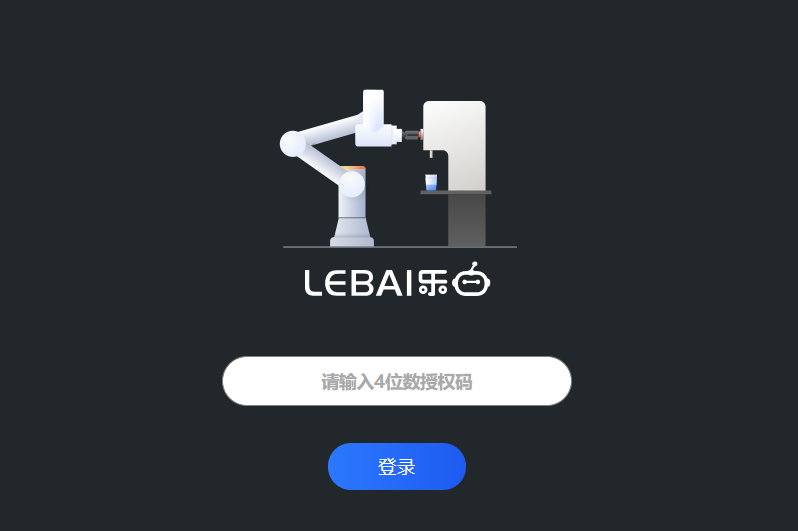
\includegraphics[width=0.8\textwidth]{screen/2-4.png}
%     \caption{登录\LM}
%     \label{fig:登录LM}
% \end{figure}

% \clearpage

\section{设置引导页}

当机器人开箱上电后,第一次登录\LM 时,首先需要按照设置引导页的提示进行初次使用的安装设置。
\subsection{系统设置}
% 第一步,
在\mnu{系统设置}中可以自定义语言、时区、时间。

\begin{figure}[ht]
    \centering
    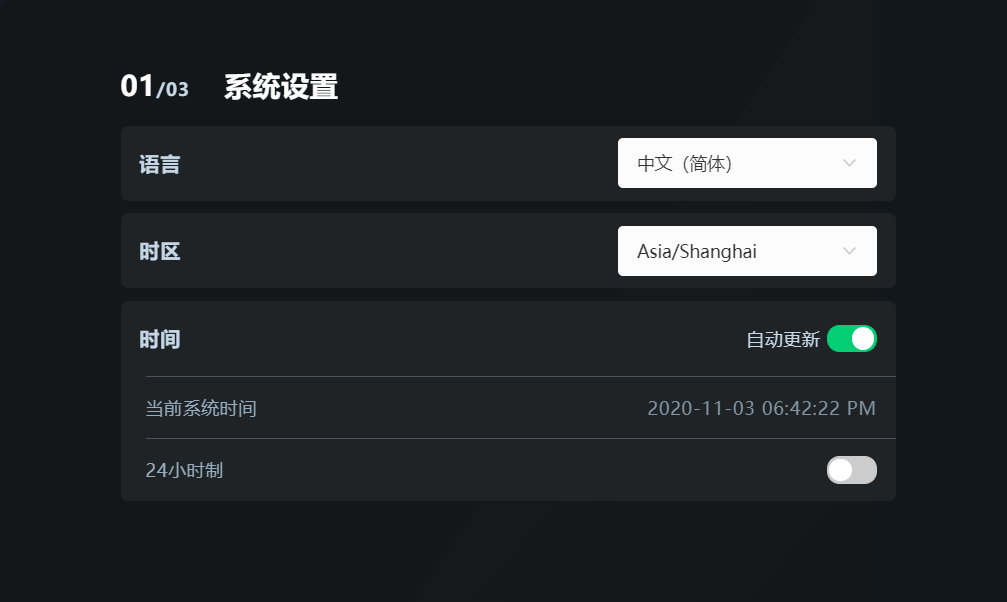
\includegraphics[width=0.8\textwidth]{screen/2-5.png}
    \caption{系统设置}
    \label{fig:系统设置}
\end{figure}

\subsection{机器人设置}
% 第二步,
在\mnu{机器人设置}中可以设置机器人的安装方式、操作模式及碰撞检测。
\begin{enumerate}
\item 安装方式

	根据实际安装方式,参照\prettyref{fig:安装方式}的“图标对照表”选择正装、倒装、侧装。

	\begin{figure}[ht]
		\centering
		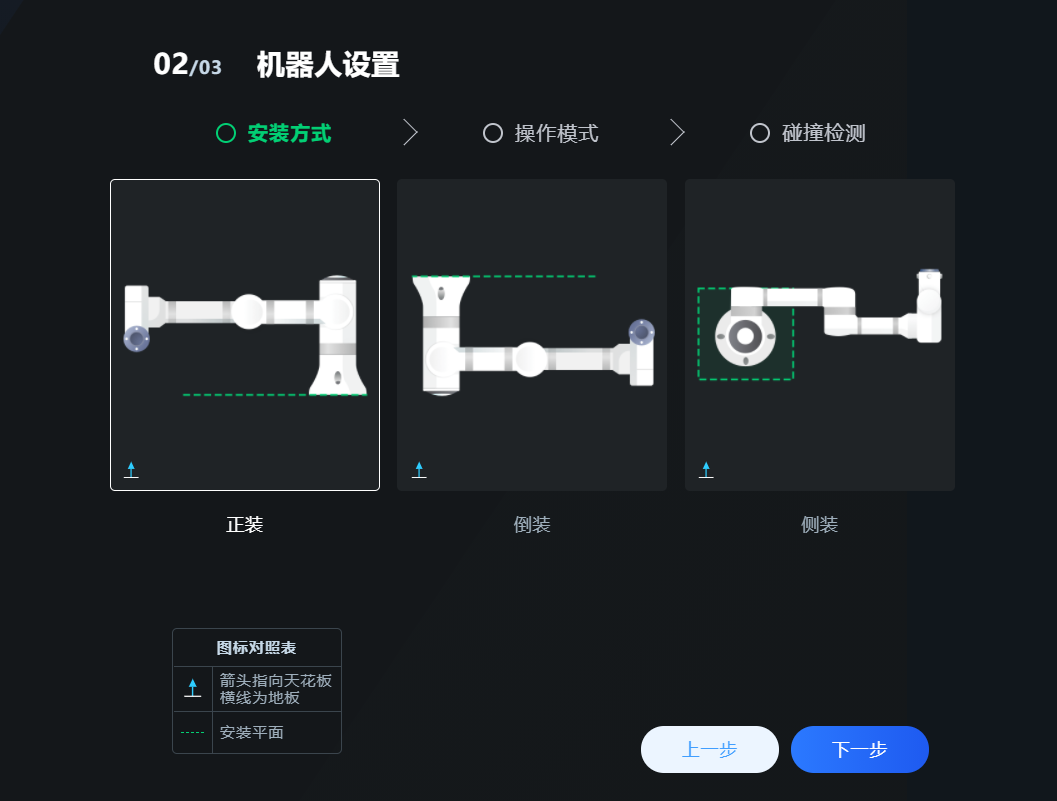
\includegraphics[width=0.8\textwidth]{screen/2-6.png}
		\caption{安装方式}
		\label{fig:安装方式}
	\end{figure}

	\danger{安装方式的选择一定要与实际安装方式一致,否则有可能导致误伤。}

% \clearpage

\item 操作模式

可在\mnu{新手模式}、\mnu{专家模式}和\mnu{维护模式}之间选择。 
\begin{itemize}
\item[新手模式] 适合没有编程基础的新手,无需理解任何逻辑和代码;
\item[专家模式] 适合有一定编程基础和逻辑基础的高级用户;
\item[维护模式] 适合日常维护人员,该模式仅包含最基础的常用操作。
\end{itemize}
您可以根据自身情况选择相应的操作模式。 

	\begin{figure}[ht]
		\centering
		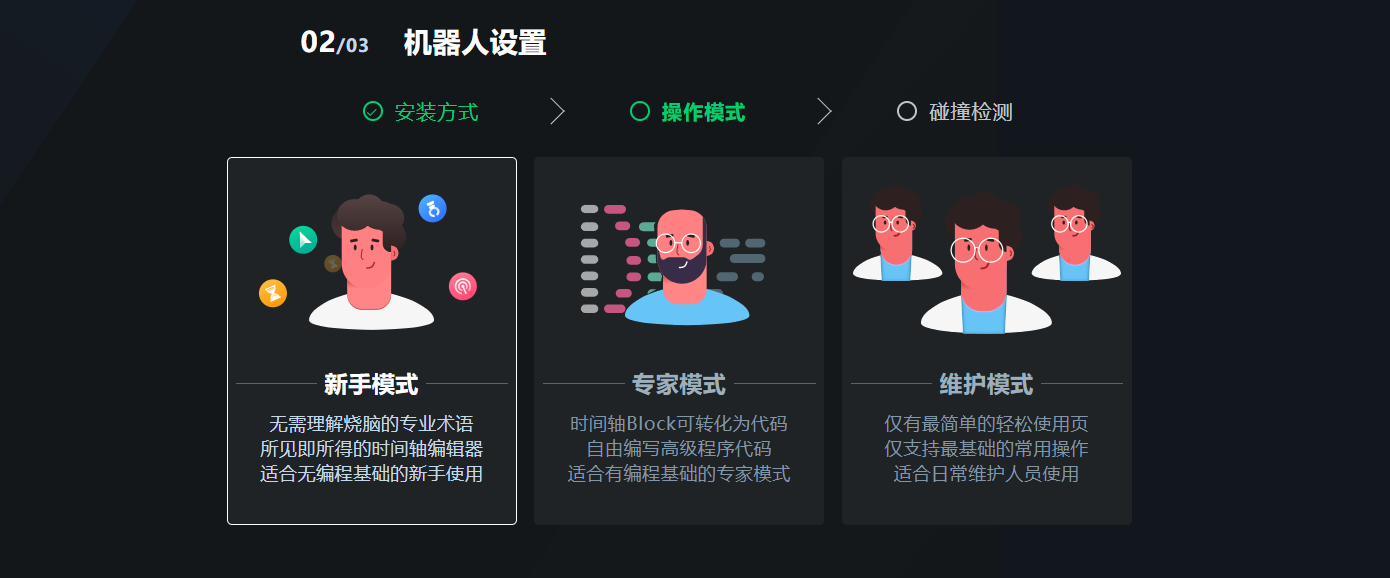
\includegraphics[width=0.8\textwidth]{image/07/图2.7 操作模式.png}
		\caption{操作模式}
		\label{fig:操作模式}
	\end{figure}

\clearpage

\item 碰撞检测

	检测开关默认为开,“碰撞后的动作”默认为\mnu{急停},可选择\mnu{急停}或\mnu{暂停},同时可以拖动拉杆来调整“检测灵敏度”大小。点击\btn{下一步},进入界面设置。

	\begin{figure}[ht]
		\centering
		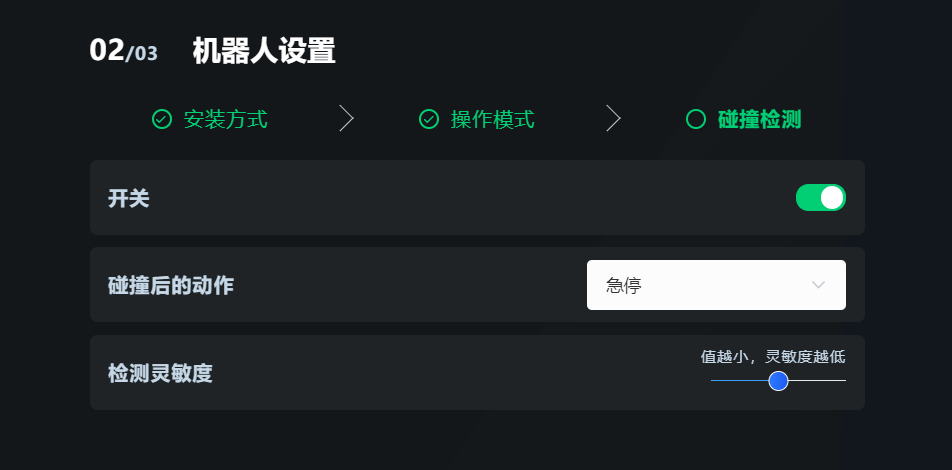
\includegraphics[width=0.8\textwidth]{screen/2-8.png}
		\caption{碰撞检测}
		\label{fig:碰撞检测}
	\end{figure}

	\danger{机器人运行过程中,无论是否开启“碰撞检测”功能,禁止在没有防护的情况下进入到机器人工作空间内\footnote{详见\prettyref{sec:工作空间}。},否则存在人员被机器人撞伤的危险。}

\end{enumerate}

% \clearpage

\subsection{界面设置}

% 第三步,
在\mnu{界面设置}中设置界面主题,推荐使用\mnu{深色主题}。
% 可以选择\mnu{深色主题}或\mnu{浅色主题},目前\LM 浅色主题还在测试阶段,

% \begin{figure}[ht]
% 	\centering
% 	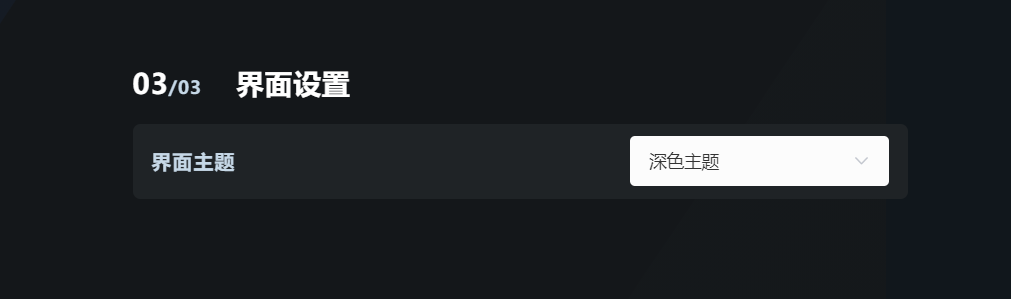
\includegraphics[width=\textwidth]{screen/2-9.png}
% 	\caption{界面设置}
% 	\label{fig:界面设置}
% \end{figure}

点击\btn{完成},进入\LM 首页。

% \clearpage

\section{首页}

在\LM 首页,页面分为:左面板、状态区、控制区、主功能入口、任务历史、底部控制箱以及顶部标题栏七个区域。急停按钮和胶囊控制区可通过长按拖动调整位置。

\begin{itemize}
	\item 左面板显示机器人当前的坐标位置和姿态数据,关节空间的关节角度数据、末端负载的质量与质心、工具中心点(TCP)的位置和姿态数据、整机温度数据。左面板单个及全部菜单项均可展开/隐藏。
	\item 状态区显示机器人的实时状态。 
	\item 控制区包含机器人的启停按钮,软件示教按钮、速度比例调整控件以及隐藏的任务暂停/恢复按钮。 
	\item 主功能入口包含场景、控制和设备三个主功能入口。 
	\item 任务历史包含所有的任务历史列表。 
	\item 底部控制箱点击展开后包含开关机按钮、无线网络IP、有线网络IP、通讯协议及电压电流信息。
	\item 顶部标题栏左侧显示机器人名称及版本号、场景、控制、设备及系统设置;右侧包含真机在线与离线仿真的切换、点单与轻松使用的功能入口、任务历史、消息中心以及退出登录。 
	\item 胶囊控制区上半部分为 状态控制 , 下半部分为 任务历史 。	
\end{itemize}

\begin{figure}[ht]
	\centering
	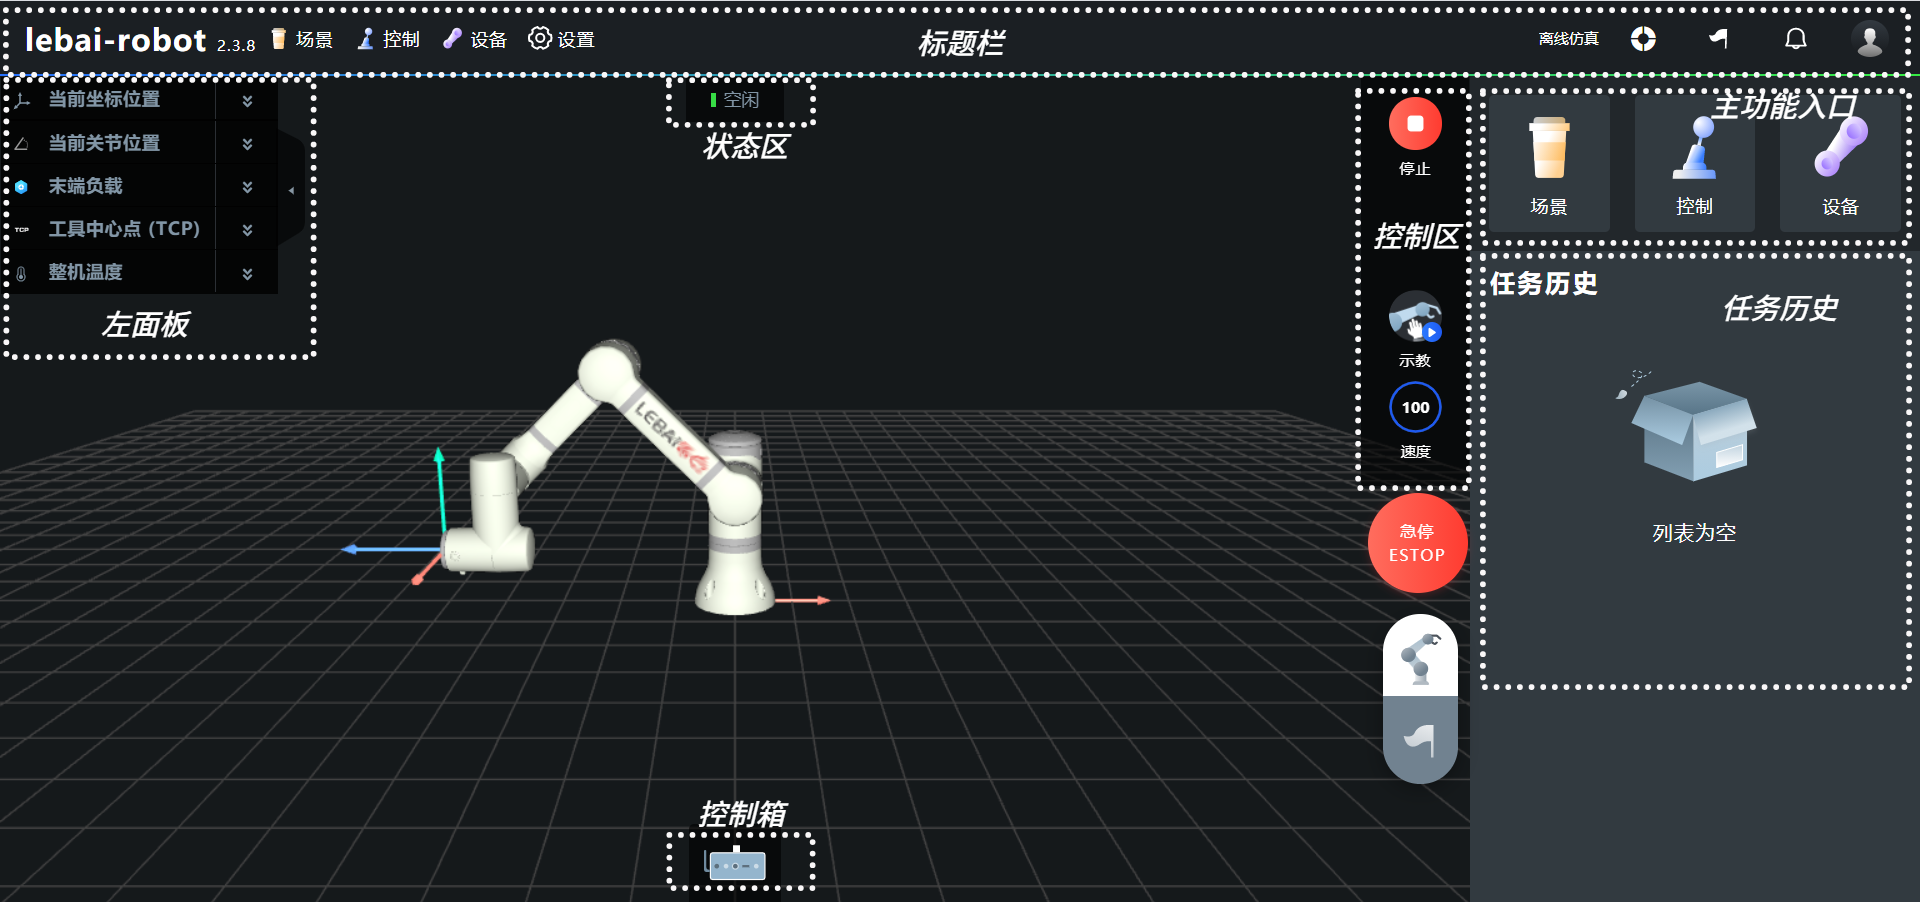
\includegraphics[width=\textwidth]{image/07/图2.10 首页 .png}
	\caption{\LM 首页}
	\label{fig:LM首页}
\end{figure}

% \clearpage

\subsection{机器人状态}

机器人状态区显示机器人当前状态,具体说明可参考\prettyref{tab:机器人状态列表}。

\begin{table}[ht]
    \centering%\small
	\rowcolors{1}{trEven}{trOdd}
    \caption{机器人状态列表}
	\def\Robot{机器人}
    \begin{tabular}{cll}
\rowcolor{th} \Th{状态码} & \Th{状态} & \Th{说明}\\
-1 & 控制系统故障 & \Robot 软件控制系统异常\\
0 & 硬件通讯故障 & \Robot 硬件通讯故障\\
1 & 已急停 & \Robot 处于急停状态,请确认安全性\\
2 & 初始化中 & \Robot 初始化中\\
4 & 初始化完成 & \Robot 电源已开启\\
5 & 空闲 & \Robot 处于空闲状态\\
6 & 暂停 & \Robot 处于暂停中状态\\
7 & 运行中 & \Robot 运行中\\
8 & 更新中 & \Robot 系统更新中\\
9 & 启动中 & \Robot 初始化完成到空闲的启动过程中\\
10 & 正在停止 & \Robot 空闲状态转到停止状态\\
11 & 示教中 & \Robot 处于示教模式中\\
12 & 已停止 & \Robot 处于停止状态,非急停状态\\
    \end{tabular}
    \label{tab:机器人状态列表}
\end{table}

\subsection{位置信息}
\LM 首页左面板实时同步机器人位置信息,包含坐标空间和关节空间。如\prettyref{fig:位置信息},当前坐标位置显示机器人在坐标空间的位置和姿态的实时数据;当前关节位置显示机器人 6 个关节角度的实时数据。

\begin{figure}[htb]
	\centering
	\begin{minipage}[t]{0.3\linewidth}
		\centering
		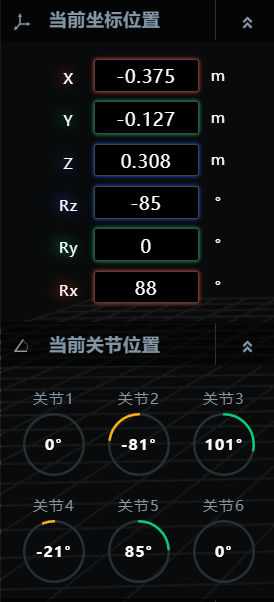
\includegraphics[width=3cm]{image/07/图2.11 位置信息.png}
		\caption{位置信息}
		\label{fig:位置信息}
	\end{minipage}
	\hfill
	\begin{minipage}[t]{0.3\linewidth}
		\centering
			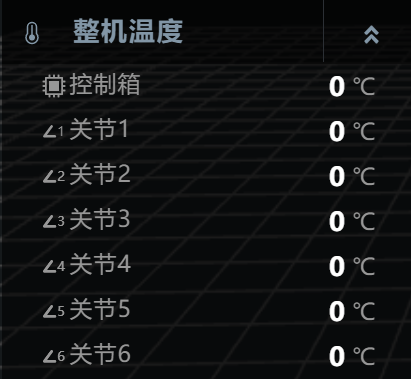
\includegraphics[width=3cm]{image/07/图2.12 整机温度.png}
			\caption{整机温度}
			\label{fig:整机温度}
	\end{minipage}
	\hfill
	\begin{minipage}[t]{0.3\linewidth}
		\centering
		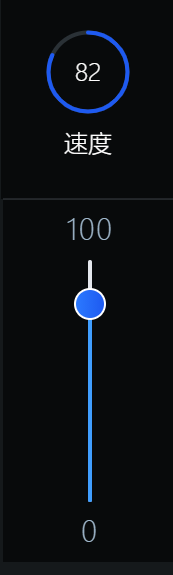
\includegraphics[height=4cm]{screen/2-13.png}
		\caption{速度比例}
		\label{fig:速度比例}
	\end{minipage}
\end{figure}

\subsection{温度信息}
如\prettyref{fig:整机温度},
\LM 首页左面板实时显示机器人的控制箱温度以及每个关节的实时温度。每个关节正常温度在室温至$65\oC$之间。

\danger[警告]{当关节温度显示超过$65\oC$时,请勿触摸机器人外表面,否则有高温烫伤风险,并请立即停机,待机器温度回到常温,再检查当前机器人负载是否超过额定有效负载$3\kg$或机器人是否碰撞外部物品。}

\subsection{速度比例}
% 点击\LM 首页控制区的速度图标,在展开的滑动条中拖动滑块或点击滑动条以调整机器人的运行速度比例,比例范围为$0\sim 100$。
点击\LM 首页控制区的速度图标,在如\prettyref{fig:速度比例}展开的滑动条中拖动滑块或点击滑动条以调整机器人的运行速度比例,比例范围为$0\sim 100$。 

\subsection{消息中心}
在消息中心中,可查看机器人提示、警告、软硬件异常的消息通知。鼠标点击\LM 首页右上角的消息图标\colorbox{black}{\icn{image/22.pdf}}可以打开消息中心。

\begin{figure}[htb]
	\centering
	\begin{minipage}[t]{0.5\linewidth}
		\centering
		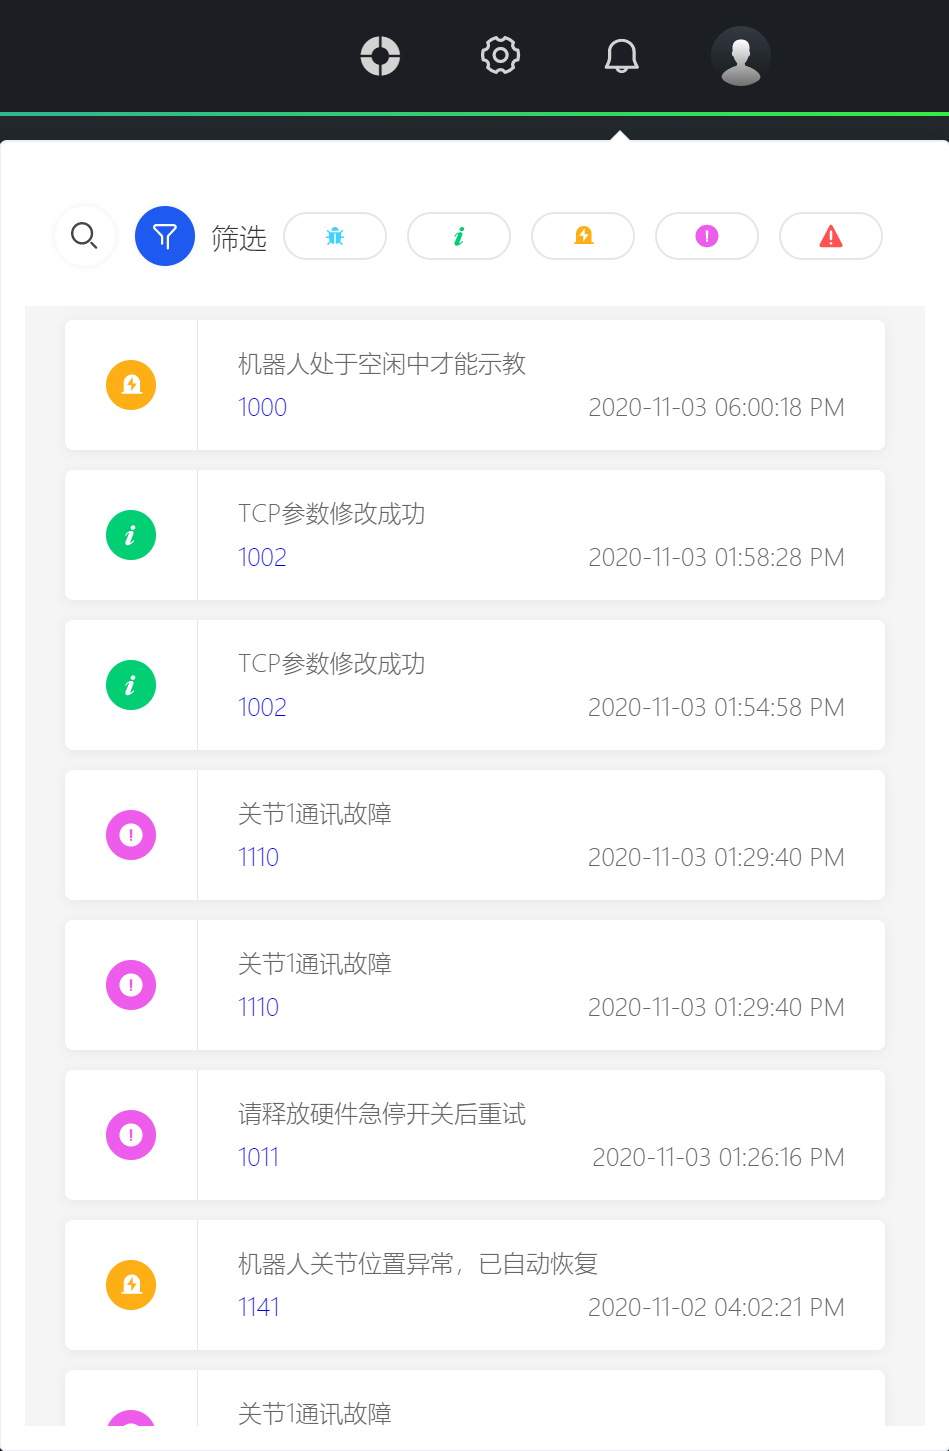
\includegraphics[width=4cm]{screen/2-14.png}
		\caption{消息中心}
		\label{fig:消息中心}
	\end{minipage}
	\hfill
	\begin{minipage}[t]{0.45\linewidth}
		\centering
		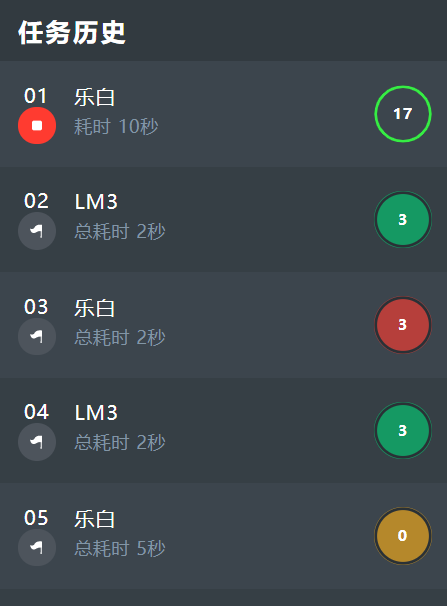
\includegraphics[width=4cm]{image/07/图2.13 任务历史.png}
		\caption{任务历史}
		\label{fig:任务历史}
	\end{minipage}
\end{figure}
在消息中心中,有以下两种方式进行消息搜索:
\begin{enumerate}
	\item 通过关键字搜索消息通知。
	\item 通过筛选以下类型的消息通知:
	\begin{itemize}
% \item[\icn{image/30.pdf} 调试]
\item[\icn{image/29.pdf} 信息] 信息提醒类消息;
\item[\icn{image/28.pdf} 警告] 系统运行时警告级别的提醒,一般不影响使用;
\item[\icn{image/27.pdf} 错误] 系统出现了错误,需要保持关注错误的发生概率,如果频繁发生,需尽快点击查看解决方案或与本公司及时取得联系;
\item[\icn{image/26.pdf} 致命] 系统出现严重错误,存在运行风险或已无法正常运行,此时必须立即停机,查看解决方案或与本公司及时取得联系。
	\end{itemize}
\end{enumerate}

如\prettyref{fig:消息中心},
% 点击消息项内容左下角的错误码超链接,
单条消息左下角的数字为错误码,点击错误码链接可跳转至本公司官网对应的错误码解决方案页面,在该页面中可根据错误码查找对应的问题解释及解决方案。

\subsection{任务历史}
\label{sec:任务历史}
在 \LM 首页,或者点击标题栏小旗帜按钮,可以查看任务历史。

任务历史列表中显示正在运行中及已完成的任务,包含每个任务的名称、花费时长、运行次数及状态,并以时间顺序排列展现。

\begin{itemize}
	\item 当任务正在运行时,左侧显示任务中止按钮,右侧运行状态显示蓝色; 
	\item 当任务已完成,左侧显示重新运行按钮\icn{image/icon_flag.pdf},点击可重新运行当前选择的任务。右侧状态栏为绿色表示任务已完成;黄色表示任务已中止;红色表示任务已急停。
\end{itemize}

点击\mnu{任务历史}中的任务名称,可进入该任务对应的场景编辑页面。

\danger[警告]{运行某个场景,则该场景的任务进入任务历史列表。当该任务完成后,点击 重新运行 按钮,当前执行的任务为之前执行该任务的场景数据,重新运行的任务不受场景的数据变更影响,以上一次运行任务的场景数据为准。}

\subsection{离线仿真}

点击标题栏按钮可以将系统切换离线仿真模式与真机在线模式,切换过程中会重启软件系统。

\begin{itemize}
\item \mnu{真机在线}模式是通过软件系统直接操作机器人执行任务。
\item \mnu{离线仿真}即脱机操作,使用系统界面的仿真机器人模型进行模拟操作。
\end{itemize}

% \clearpage

\section{启动机器人}
进入\LM ,如\prettyref{fig:启动机器人}所示,点击控制区的启动按钮;经过短暂的\mnu{启动中},首页状态区转为\mnu{空闲},表示您已成功启动机器人。

\begin{figure}[ht]
	\centering
	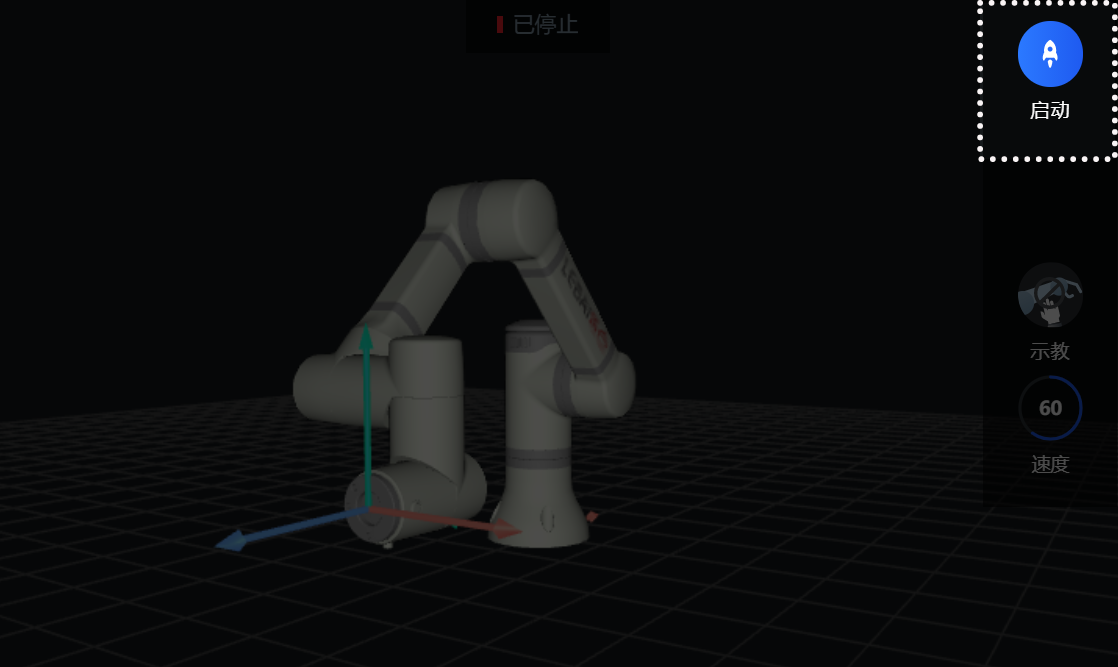
\includegraphics[width=\textwidth]{image/07/图2.17 启动机器人.png}
	\caption{启动机器人}
	\label{fig:启动机器人}
\end{figure}

\section{停止机器人}
当机器人处于\mnu{运行中}或\mnu{空闲}状态时,可以点击首页或如\prettyref{fig:胶囊控制区}所示的胶囊控制区的红色停止按钮;经过短暂的\mnu{停止中},当机器人状态变为\mnu{已停止}时,表示您已成功停止机器人。

% \begin{figure}[ht]
% 	\centering
% 	\includegraphics[width=\textwidth]{image/6.pdf}
% 	\caption{\LM  首页--停止机器人}
% 	\label{fig:停止机器人}
% \end{figure}

\section{急停机器人}

% 急停操作有两种方式,可任选其一:
\begin{itemize}[leftmargin=3.5em]
	\item[软急停] \LM 右下方的红色\btn[Danger]{急停ESTOP}按钮;
	\item[硬急停] 按下控制箱顶部的急停按钮(红色凸起按钮)或外接急停按钮(选配)。
\end{itemize}

\info{使用硬急停操作后,急停操作不会自动释放,需要顺时针旋转急停按钮,解除锁定后完成释放。}

\section{关闭机器人}
\begin{enumerate}
	\item 先停止或者急停机器人。 
	\item 关闭操作有两种方式,可任选其一: 
	\begin{itemize}
	\item 软关闭:选中\LM 首页下方的控制箱图标,点击翻转展开后最左侧的关机按钮。
	\item 硬关闭:长按控制箱开关机按钮或使用外置开关机按钮(选配),直至控制箱开关机按钮的蓝色指示灯熄灭。 
		\end{itemize}
	\item 关闭控制箱背板的红色总电源开关。 
\end{enumerate}

\danger[警告]{关闭机器人需严格遵守上述操作步骤,否则可能导致机器人文件系统损坏、机器人功能故障等问题。}

% \section{胶囊控制区}
% 胶囊控制区仅在非首页时显示,胶囊上半部分为\mnu{状态控制},胶囊下半部分为\mnu{任务历史}。长按胶囊本体可拖动调整胶囊控制区在页面中的位置。

% \begin{figure}[hb]
% 	\centering
% 	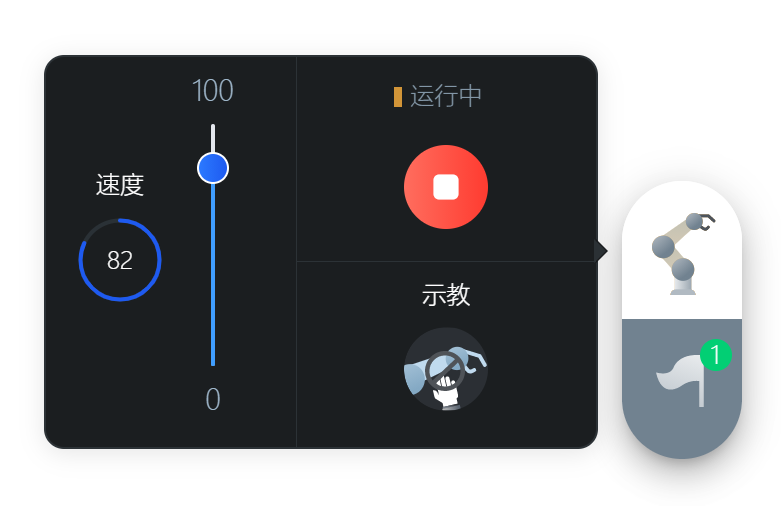
\includegraphics[height=4cm]{screen/2-18.png}
% 	\caption{胶囊控制区}
% 	\label{fig:胶囊控制区}
% \end{figure}

% \begin{itemize}[leftmargin=4.5em]
% 	\item [状态控制] 包含机器人当前状态、机器人启动/停止按钮、示教按钮以及速度调整拉杆,可以在非首页时操作和控制机器人。
% 	\item [任务历史] 包含正在运行中及已完成的任务列表、任务的暂停/恢复和停止按钮,可以在非首页时查看任务历史,具体操作见\prettyref{sec:任务历史}。
% \end{itemize}
